\documentclass[12pt]{article}
\usepackage[utf8]{inputenc}
\usepackage[T1]{fontenc}
\usepackage{cite}
\usepackage{graphicx}
\usepackage{float}
\usepackage{multirow}
\usepackage[table,xcdraw]{xcolor}
\usepackage[colorlinks]{hyperref}
\usepackage{epstopdf}
\hypersetup{
  colorlinks = true,
  linkcolor  = magenta,
  citecolor  = magenta
}
\usepackage[all]{hypcap}
\usepackage{listings}
\usepackage{color}
\definecolor{dkgreen}{rgb}{0,0.6,0}
\definecolor{gray}{rgb}{0.5,0.5,0.5}
\definecolor{mauve}{rgb}{0.58,0,0.82}
\lstset{frame=tb,
  language=Python,
  aboveskip=3mm,
  belowskip=3mm,
  showstringspaces=false,
  columns=flexible,
  basicstyle={\small\ttfamily},
  numbers=none,
  numberstyle=\tiny\color{gray},
  keywordstyle=\color{blue},
  commentstyle=\color{dkgreen},
  stringstyle=\color{mauve},
  breaklines=true,
  breakatwhitespace=true,
  tabsize=3
}

\title{Project Checkpoint: CSE 6730 Project 1}
\author{Chris Dunlap, Allen Koh, Matt May}
\date{Spring 2016}

\begin{document}

\begin{titlepage}
  \maketitle
  \thispagestyle{empty}
\end{titlepage}

\newpage
  \tableofcontents
  \thispagestyle{empty}
\newpage

\section{Problem Statement}
\label{sec:problem}

The efficient evacuation of physical structures is an important problem with a
long history of multi-disciplinary study \cite{zheng2009modeling}. For this
study, we focus specifically on the problem of efficiently evacuating the
area around Bobby Dodd Stadium in Atlanta, GA. Bobby Dodd Stadium, the home of
the NCAA Division-I Georgia Tech Yellow Jackets football team, has a
seating capacity of 55,000 individuals.

\begin{figure}[H]
  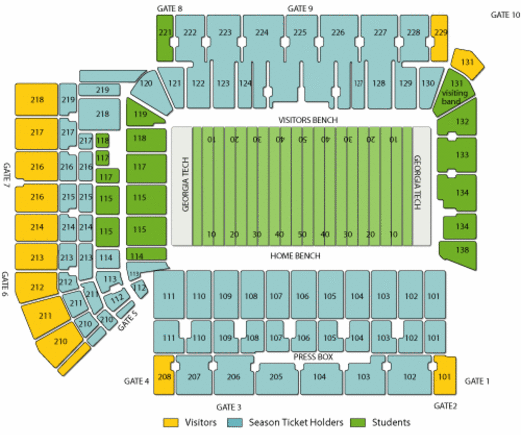
\includegraphics[width=\linewidth,natwidth=521,natheight=435]{stadium_diagram_updated.png}
  \caption{Bobby Stadium Stadium seating chart.}
  \label{fig:stadiumseating}
\end{figure}

Our primary objective in this study is to minimize the pedestrian evacuation
time of the stadium and its surrounding area as attendees leave the area
following a home football game. We do this by taking a parametric approach, in
which we explore the effects of road closures and the ``takeover'' of certain
intersections by law enforcement in promoting an optimal result.

For purposes of this study, we define the system under investigation (SUI) as a
rectangular polygon (Fig. \ref{fig:polygon}) surrounding the stadium. To be
clear, the SUI is defined as the area inside the polygon but outside the
stadium. As pedestrians exit the stadium, they enter the SUI, and as they cross
the boundary of the polygon, they exit it.

\begin{figure}[H]
  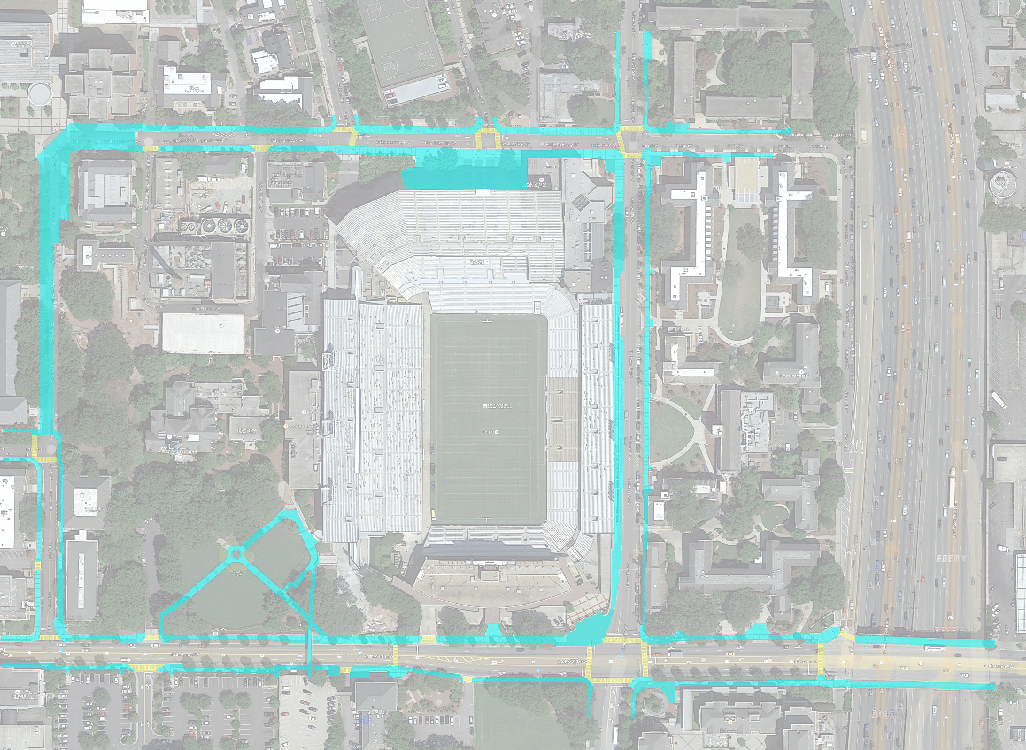
\includegraphics[width=\linewidth,natwidth=1023,natheight=750]{GATechMap_20160301.png}
  \caption{The system under investigation.}
  \label{fig:polygon}
\end{figure}

The stadium has 11 ``exit zones'' modeled that serve as ingress (pre-game) and
egress (post-game) sites. These serve as the entry points to our simulation. As
pedestrians enter the SUI, they are assigned a destination and then proceed
to their destination by way of pedestrian walking paths (i.e., sidewalks).
These are denoted as the cyan-colored portions of the SUI.  Pedestrian crosswalks
are also modeled; these are the yellow-colored portions of the SUI.

\section{Related Work}
\label{sec:literature}

A variety of techniques have been used to model pedestrian movement. Cellular
automata, lattice gas, social force, fluid-dynamic, agent-based, game-theoretic,
and animal experimentation-based approaches have been used
\cite{zheng2009modeling}. As noted by Zheng, Zhong, and Liu
\cite{zheng2009modeling}, models often encounter or attempt to model several
common phenomena: clogging, side-stepping, lane formation, and herding
behavior, among them.

These phenomena manifest themselves in different ways and at different
magnitudes depending on the system being modeled. In one of the early
explorations of 2D cellular automata for simulating traffic flow in the related
domain of vehicular traffic simulation, Biham and Middleton \cite{biham1992self}
note the presence of a sharp
\textit{jamming transition} in which all cars in the simulation transition from
moving at maximal speed to being stuck. Similar effects were noted in
simulations of bi-directional pedestrian movement, with Weifeng, Lizhong, and
Weicheng \cite{weifeng2003simulation} finding that as total pedestrian density
increases, a critical value is reached at which the system transitions into a
jammed state where only a few pedestrians are able to proceed.

In a slightly different take on the problem, Okazaki and Matsushita
\cite{okazaki1993study} modeled pedestrian evacuation using Coulomb's Law, with
actors magnetically moving toward their goals and away from obstacles that would
lead to collisions. In another application of equations of natural phenomena,
Helbing \cite{helbing1998fluid} derived fluid dynamic equations for explaining
the movement of pedestrian crowds, observing phenomena such as the development
of lanes, jamming, and crossing. Helbing \cite{helbing2000simulating} further
notes an explicit ``faster-is-slower'' effect, in which attempting to move faster
results in a lower average speed of leaving at high pedestrian density in
evacuation scenarios.

In a more recent study, Helbing et al. \cite{helbing2005self} use a
``social force'' model, which states that pedestrians operate in some sense
automatically when reacting to obstacles and other pedestrians, applying
strategies that have been learned to be most effective over time. Several
suggestions are made to alleviate the three most common problems in pedestrian
crowds: counterflows, bottlenecks, and intersecting flows. The presence of
strategically placed obstacles are found to actually reduce these negative
phenomena, leading to improved flow.

Building on previous cellular automata-based models, Burstedde et al.
\cite{burstedde2001simulation} introduce a \textit{floor field}, a secondary
grid of cells which underlies the main grid and acts as a substitute for
pedestrian intelligence. These fields can be either static or dynamic, and are
capable of promoting the avoidance of jams, as well as simulating attractive
effects, in which pedestrians are more likely to follow in the paths of
pedestrians ahead of them.

Taking a more algorithmic approach, Fang et al. \cite{fang2011hierarchical} have
designed a modified ant colony optimization (ACO) algorithm for optimizing
pedestrian evacuation, seeking to minimize evacuation time, evacuation distance,
and congestion. Kemloh Wagoum, Seyfried, and Holl \cite{kemloh2012modeling}
utilize an observation principle approach in modeling pedestrian evacuation,
in which pedestrians first observe their environment and then make a final
decision on strategy based on obtained data.

There are several takeaways from the literature described above that have
potential applicability to the model at hand. First, on the topic of modeling
pedestrian walkways, several papers focused on either a single passageway,
enclosed areas with obstacles (walls, pillars, etc.), or evacuation from a
room with a single doorway. However, modeling walkways as an undirected graph
\cite{fang2011hierarchical} seems feasible given the problem at hand, where
there are multiple pathways one can take to get to a single destination. In
papers where cellular automata was utilized, the median size of each cell on the
walkway was 0.4m\textsuperscript{2}
\cite{blue2001cellular,burstedde2001simulation,weifeng2003simulation}.

Second, on the topic of pedestrian modeling, multiple walking speed techniques
were used, ranging from a constant speed of 1 m/s \cite{weifeng2003simulation}
or 1.3 m/s \cite{burstedde2001simulation}, to using a distribution resembling a
step function \cite{blue2001cellular} or a Normal distribution
\cite{klupfel2005models}. In either distribution, the median walking speed was
also approximately 1.3 m/s. For reaction to stimuli, 0.3 seconds was utilized
\cite{burstedde2001simulation}, which was one time step in that particular
simulation. Incorporation of opportunistic side-stepping was done
\cite{blue2001cellular}, in addition to using least-cost algorithms for
establishing the path a pedestrian would like to take
\cite{fang2011hierarchical}. In the context of cellular automata, analyzing a
given pedestrian's cell's neighbors in either a 4-connected
\cite{weifeng2003simulation} or 8-connected fashion
\cite{burstedde2001simulation} to decide in which direction the pedestrian would
like to walk for the next time step was utilized. This, coupled with a dynamic
floor field \cite{burstedde2001simulation} to factor in long-distance forces,
could be utilized. In cases where there are two pedestrians targeting each other's
current positions for a next move, which may happen when they are walking in
opposing directions in the same lane, the concept of \textit{place exchange}
has merit when two pedestrians walking in opposing directions \cite{blue2001cellular}.

Finally, simulation execution practices were also gleaned. Care must be taken
to do parallel-based updating to avoid sequential updating from interfering with
underlying model execution \cite{blue2001cellular}. The practice of using
a deterministic model running with randomized initial conditions has precedent
\cite{biham1992self}. Finally, to achieve statistical significance, 20 runs per
configuration has been used \cite{blue2001cellular}.

\section{Conceptual Model}
For our simulation, we utilize a 2-dimensional cellular automata (CA)-based
approach. We construct a discrete time-stepped model, in which the simulation
clock advances by a fixed interval every time step. In our simulation, 1 time step is modeled as 1 second. We utilize a stochastic
(probabilistic) approach, in which the output of each individual simulation
run is a random variable. Thus, multiple simulation runs will be performed and
statistical analysis will be used to provide confidence levels in our results.

\subsection{Inputs}
The primary input to our simulation model is a stream of football game attendees
(i.e., pedestrians) exiting Bobby Dodd Stadium following a home football game.
For purposes of modeling this input stream, we assume pedestrian interarrival
time at the stadium gate boundary is a homogeneous stochastic process that
follows a Poisson distribution, as has been used in the literature
\cite{rahman2013modelling}. Empirically, we determined the mean number of
pedestrians per second arriving at the exit boundary from a 5-meter-wide exit to
a stadium to be 4.05. This was determined by observing the number of pedestrians
exiting a stadium on video \cite{youtubestadium}. This value was then used as
the basis for the lambda-parameter used for sampling of the Poisson
distribution. This provides a stream of exiting pedestrians in which the number
of pedestrians exiting at any given second is independent of the pedestrians
exiting at the previous second. While this assumption is reasonable for an
initial simulation model, it should be noted that in reality there is likely
some variation over time. We use a simple queue structure to model the entry of
pedestrians into our simulation. As pedestrians arrive at the gate boundary and
exit the stadium, they enter the SUI.

The random number generator used to sample the Poisson distribution underwent a
chi-squared goodness-of-fit test to evaluate the hypothesis that the numbers obtained
were indeed following a Poisson distribution. A 7-bin histogram of 1771 observed
values from the generator, along with the corresponding theoretical histogram,
is shown in Fig. \ref{fig:poissoncompare}. The chi-squared statistic was 1.2640;
when compared with the critical value of 11.0705 (from chi-squared distribution
with 5 degrees of freedom and 0.05 level of significance), the hypothesis
stating that the distribution is Chi-Squared is not rejected.

\begin{figure}[H]
  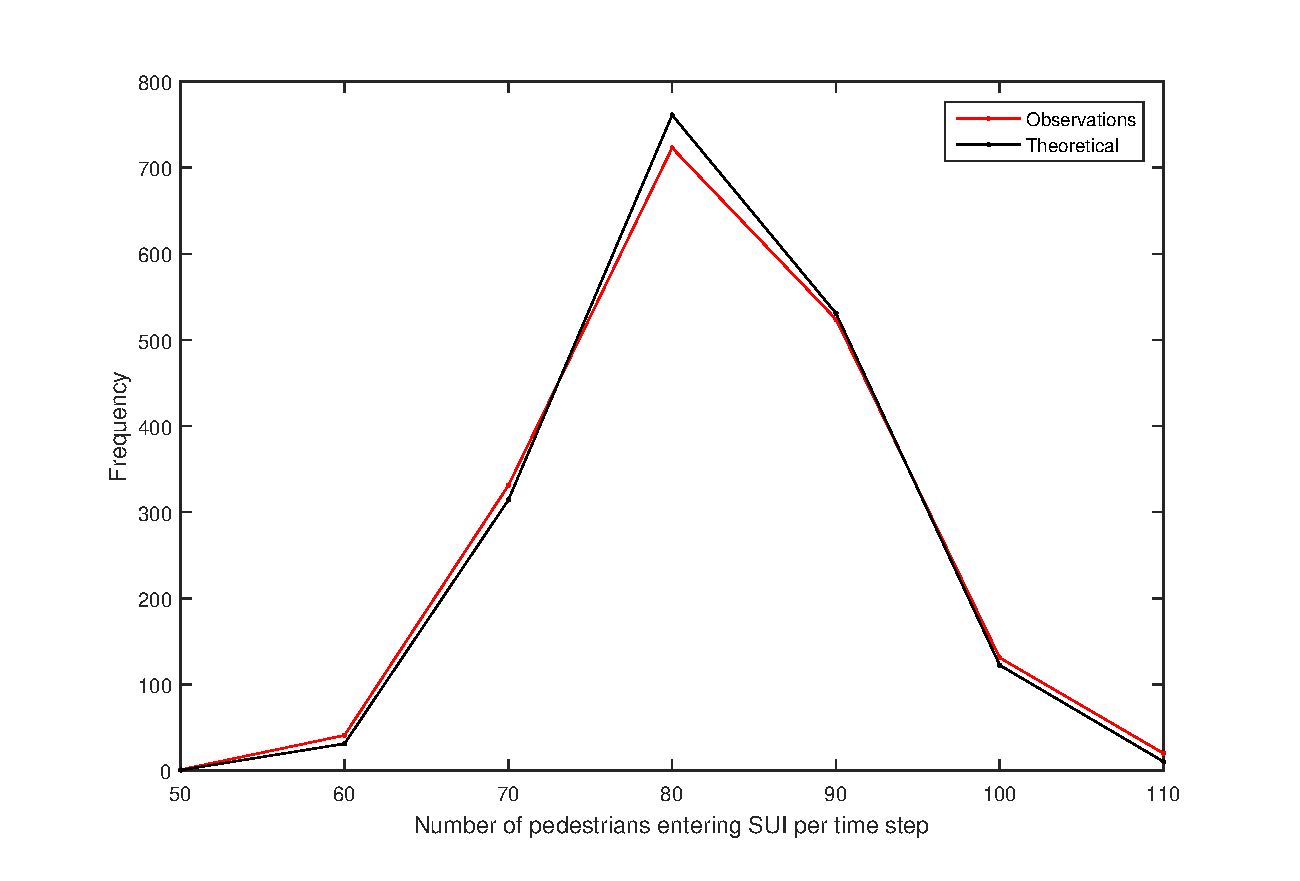
\includegraphics[width=\linewidth,natwidth=811,natheight=512]{PoissonCompare.eps}
  \caption{Poisson PDF Chi-Squared Test ($\lambda$ = 82.4280).}
  \label{fig:poissoncompare}
\end{figure}

In addition, we select each pedestrian's target destination and walking
speed at random. For selecting a target destination, we assume that pedestrian
destinations are uniformly distributed and sample from a pool of exit nodes
from the SUI that correspond to parking lots, local housing, and public
transportation. For determining a walking speed for each pedestrian, we sample
from a distribution previously referenced in the literature by Blue and Adler
\cite{blue2001cellular} (5\% fast walkers (4 cells/time step), 90\% standard
(3 cells/time step), 5\% slow (2 cells/time step)).

Pedestrians in our model can be considered a consumer entity class
\textit{Pedestrian} with attributes which will be set and updated during the
course of our simulation. Table \ref{table:ped} provides an overview of the
attributes of the \textit{Pedestrian} class.

\def\arraystretch{1.5}
\begin{table}[hb!]
  \centering
    \begin{tabular}{p{0.3\linewidth}p{0.6\linewidth}}
     \hline
     Attribute & Description \\
     \hline
     Current        & \textit{Node} object corresponding to the current
                      location of the pedestrian. \\
     Destination    & \textit{Node} object (see Table \ref{table:node})
                      corresponding to the final destination of the
                      pedestrian. \\
     TargetNext     & The desired next node to move to in the pedestrian's
                      shortest path to his destination, as computed by
                      Dijkstra's algorithm. \\
     Speed          & Walking speed, formulated in grid cells traversed per
                      time step. \\
     EgressComplete & A boolean value. This value is false when the pedestrian
                      has not yet egressed, and true when egress is complete. \\
     ShortestPath & List of node ids, corresponding to the shortest path to the
                    pedestrian's destination. \\
     \hline
    \end{tabular}
    \caption{Attributes of the \textit{Pedestrian} entity class.}
  \label{table:ped}
\end{table}

New instances of the \textit{Pedestrian} class are created and initialized
as pedestrians exit the stadium.

\subsection{Output}
For each simulation run, when all pedestrians are evacuated from the SUI we
determine the simulation to be complete. As this is a stochastic simulation,
the output results must be interpreted as samples of a random process.

At the conclusion of a series of simulation runs for a given set of parameters,
we compute an average of the total egress duration across all runs from that
series. More formally, the average egress time $E_{avg}$ for $n$ simulation runs
can be represented as:

\begin{equation}
E_{avg} = \frac{1}{n}\sum\limits_{i=1}^n d_i
\end{equation}

where $d_i$ is the total egress duration of the $i$th simulation run. This
output can be considered a derived scalar output variable (DSOV). We then
define the optimal parameter strategy to be the set of parameters $P$ that
give the the minimum value of $E_{avg}$. Confidence intervals of 90\% are also
computed to provide context on the probable range of $E_{avg}$ across all
parameters in $P$.

\subsection{Content}

\subsubsection{Approach}
Pedestrians enter the SUI from one of 11 potential entrance zones, shown in
Fig. \ref{fig:mapentranceexits}. To build the simulation space, we overlay a
2-dimensional cellular automata grid on a map of the SUI. We do this by modeling
the SUI as an undirected weighted graph. In our case, the edge weights correspond
to the spatial distance between two nodes \cite{west2001introduction}. Note
that in this section, the terms ``cell'' and ``node'' are used interchangeably.

\begin{figure}[t]
  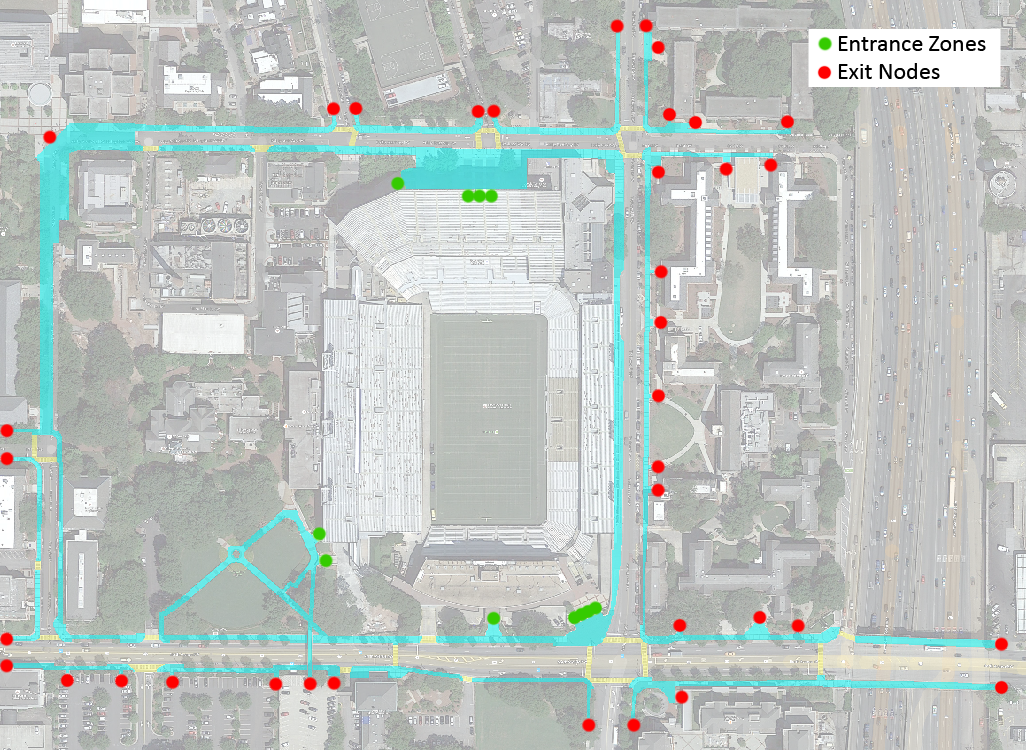
\includegraphics[width=\linewidth,natwidth=1026,natheight=750]{GATechMap_20160301_EntranceExits.png}
  \caption{SUI Entrances and Exits.}
  \label{fig:mapentranceexits}
\end{figure}

As pedestrians exit the stadium (and thus enter the SUI), they are
probabilistically assigned one of the graph's destination nodes (exit nodes
in Fig. \ref{fig:mapentranceexits}) according to a uniform distribution. When
a pedestrian reaches a destination node, that constitutes exiting the SUI.
Destination nodes were determined based on their spatial meaning when overlaid
on a map of the SUI, and constitute one of three possible classes: on-campus
housing (dormitories), parking lots, or the North Avenue Metropolitan Atlanta
Rapid Transit Authority (MARTA) station.

\def\arraystretch{1.5}
\begin{table}[hb!]
  \centering
    \begin{tabular}{p{0.3\linewidth}p{0.6\linewidth}}
     \hline
     Attribute & Description \\
     \hline
     NodeID      & Unique identifier for the node. \\
     XCoordinate & X-coordinate of the node on the 2-dimensional grid. \\
     YCoordinate & Y-coordinate of the node on the 2-dimensional grid.
                   (Note: for purposes of this simulation, the y-axis is
                    inverted.) \\
     PixelX      & X-coordinate of the node in 2-dimensional pixel space, for
                   plotting on top of a map of the SUI. \\
     PixelY      & Y-coordinate of the node in 2-dimensional pixel space, for
                   plotting on top of a map of the SUI. \\
     Paths       & A dictionary (hash map) relating each possible destination
                   to the shortest path as determined by Dijkstra's algorithm.\\
     Neighbors   & Array of \textit{Node} objects corresponding to nodes that are
                   one edge away from the node. \\
     Available	 & Boolean value indicating whether the node is available for a
                   pedestrian (true) or not available (false). \\
     NodeType    & Enumeration of the type of node, corresponding to its
                   spatial significance. The NodeType can be one of four
                   possibilities: sidewalk, road, SUI entrance, or SUI exit. \\
     CurrentPed & Pedestrian currently occupying the node, if any. \\
     \hline
    \end{tabular}
    \caption{Attributes of the \textit{Node} class.}
  \label{table:node}
\end{table}

Each node in the graph is a member of a \textit{Node} class, which
has attributes as shown in Table \ref{table:node}. As part of the simulation
initialization, the node and edge information is
populated. We define a few key types of nodes, such as entrance, exit (or
destination), and sidewalk nodes. For each entrance node $N_e$ in the graph, we
precompute the least-cost path to every possible destination node $N_d$.
In general,
we can compute the shortest path between any given node $N_i$ and destination
node $N_d$ using Dijkstra's well-known algorithm \cite{dijkstra1959note}. In our
simulation, we use a publicly available Python implementation of Dijkstra's
algorithm \cite{eppstein-dijkstra}. As pedestrians are initialized and added to
the simulation, they are randomly assigned an entrance node according to a
uniform distribution. The pedestrian then ``looks up'' the appropriate path
to the assigned destination. This path is then stored as a list structure on the
pedestrian called \textit{ShortestPath}.

At each time step, the simulation pops an element (which corresponds to a node)
from each active pedestrian's \textit{ShortestPath} attribute, and then attempts
to move the pedestrian to the given node. This repeated process drives the
pedestrian's instinct to move toward their destination, based strictly on the
shortest distance walk from their current position to their destination node.

It will likely occur that more than one pedestrian $Ped_A$ will decide to pursue
a node $N_B$ that is already occupied by a pedestrian $Ped_B$. In such cases, a
check is first performed to see if $Ped_B$ is attempting to move to the location
occupied by $Ped_A$; if so, the \textit{place exchange} logic
\cite{blue2001cellular}
is activated, and the pedestrians trade places. However, supposing the
\textit{place exchange} logic is not triggered, then an empty neighbor $N_E$ of
$Ped_A$ is chosen as the next node to move to instead. $Ped_A$ moves to $N_E$ and
the \textit{ShortestPath} list of $Ped_A$ is expanded to include the steps
that must be taken to get from $N_E$ to $N_B$, such that the path from $N_B$ to
the final destination remains intact.  If there are no empty neighbors, then
$Ped_A$ does not move at all.

\subsubsection{Parameters}

To optimize the egress of pedestrians from the SUI, there are
several parameters that can be altered. The first parameter is opening certain
streets or intersections meant for vehicular traffic and making them for use by
pedestrians only (i.e., roads become sidewalks). The second is closing certain
streets or intersections and making them for use by vehicles only (i.e.
intersections become roads). The optimal time for all pedestrians to evacuate
the SUI could be a combination of the two parameters. For example, opening an
intersection to pedestrians only and closing a nearby small intersection may to
pedestrian traffic (i.e., opening it to vehicular traffic only) may be a
combination that produces better results than only directing pedestrians to a
regular crosswalk. We explore these types of permutations in our results.

To simulate these parameters, in addition to a \textit{Node} class, there is
also an \textit{Intersection} class, which has attributes as shown in Table
\ref{table:intersection}.

\def\arraystretch{1.5}
\begin{table}[hb!]
  \centering
    \begin{tabular}{p{0.3\linewidth}p{0.6\linewidth}}
     \hline
     Attribute & Description \\
     \hline
     IntId & Integer value. A unique identifier for the intersection. \\
     Nodes & Array of \textit{Node} objects corresponding to nodes
             that are part of this intersection. \\
     IsOpen  & Boolean value indicating whether the intersection is open
             for pedestrian access (true) or not open (false). \\
     \hline
    \end{tabular}
    \caption{Attributes of the \textit{Intersection} class.}
  \label{table:intersection}
\end{table}

Intersections are modeled by mapping a given intersection ID (\textit{IntId})
to the nodes that comprise it. The intersection is therefore made up of a
group of nodes. To simulate the crosswalk opening and closing, the nodes will
be either forced closed or available for pedestrians to occupy them. If the
road is closed and vehicles are passing, then no nodes in the intersection
will be available for pedestrians.

One parameter in the simulation that can be modified is determining which
intersections will always be open to pedestrian use (i.e., closed to vehicles).
To model this case, all nodes in that intersection will behave
in the same way as the nodes that make up the sidewalk. There will be no need to
create an intersection object for that intersection. On the other hand, if there
is an intersection that is closed off for pedestrians and only available for
vehicular traffic, then the initial creation of nodes will not include that
intersection - there will be no nodes at that intersection as no pedestrian can
ever occupy those nodes.
For normal intersections, an intersection object is created and a time is
assigned to the intersection which defines the number of simulation timesteps
before changing the state of the intersection (open or closed). Fig.
\ref{fig:intersectionMap} displays the intersections and their corresponding
IDs. Table \ref{table:intersectionTimes} defines the open/close timesteps for
each intersection. These times were selected based on the size of the
intersections and the importance of the roads associated with those
intersections.

\begin{figure}[H]
	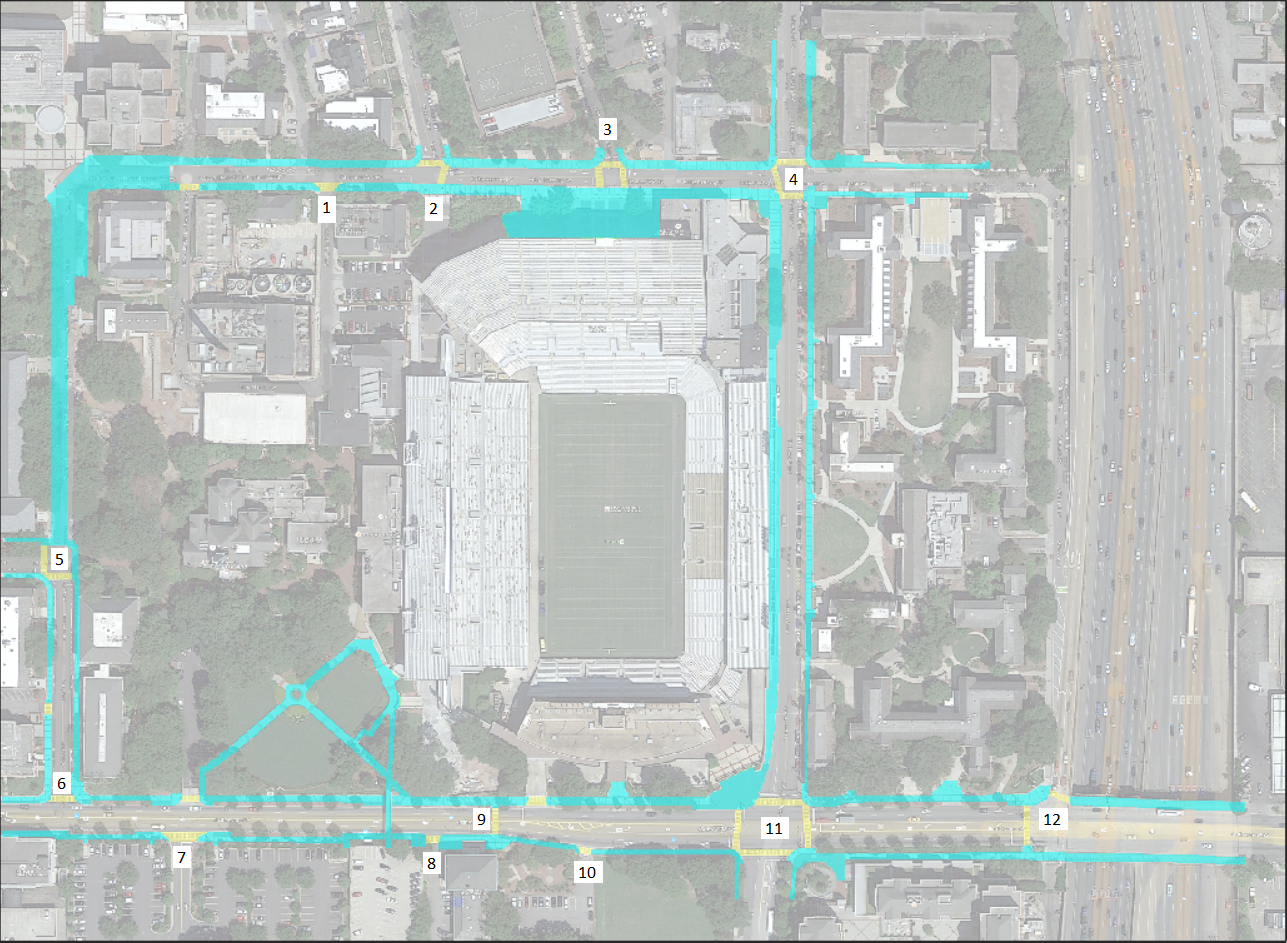
\includegraphics[width=\linewidth,natwidth=1026,natheight=750]{GATechMap_IntersectionIDs.png}
	\caption{SUI Intersection IDs.}
	\label{fig:intersectionMap}
\end{figure}

\begin{table}[t]
	\centering
	\resizebox{\columnwidth}{!}{%
	\begin{tabular}{r|c|c|c|c|c|c|c|c|c|c|c|c|}
		\cline{2-13}
		Intersection ID & \textbf{1} & \textbf{2} & \textbf{3} & \textbf{4} & \textbf{5} & \textbf{6} & \textbf{7} & \textbf{8} & \textbf{9} & \textbf{10} & \textbf{11} & \textbf{12} \\ \cline{2-13}
		Timesteps        & 15         & 20         & 25         & 30         & 25         & 20         & 15         & 15         & 20         & 15          & 40          & 25          \\ \cline{2-13}
	\end{tabular}%
}
	\caption{Intersection Open/Close Timesteps}
	\label{table:intersectionTimes}
\end{table}

If there are pedestrians that need to cross a normal intersection, but the
intersection is closed, then the pedestrians will not be able to advance to
their next node. This will cause a list of pedestrians to stay in their
current node until the crosswalk opens up (i.e., implicitly form a queue).
Once that occurs, then the pedestrians can continue to their next nodes.

\subsubsection{Random Numbers and Verification}
To model the egress of the stadium, we take a stochastic (probabilistic)
approach. In the context of a computer simulation, this necessitates the use of
a pseudorandom number generator.

For our simulation, we use the Lehmer random number generator
\cite{payne1969coding}, also known as the Park-Miller random number generator
\cite{park1988random}. For verification of the generator, we performed
100,000 iterations of a chi-square test procedure in which 1,000 samples were
drawn from the random number generator. For each iteration, we placed each
sample into one of 100 bins, forming a histogram. We then computed the
chi-square statistic, namely:

\begin{equation}
{\chi}^2=\sum_{i=1}^{n} \frac{(O_i - E_i)^2}{E_i}
\end{equation}

where ${\chi}^2$ is the chi-squared statistic, which asympotically approaches
a ${\chi}^2$ distribution, $O_i$ is the count of observations of type $i$,
and $E_i$ is the expected count of observations of type $i$. We determined the
chi-square critical value for 99 degrees of freedom and a $p$-value of 0.05 to be
123.225. Experimentally, our generator failed to pass the chi-square test only
4.95\% of the time over 100,000 iterations, allowing us to not reject the null
hypothesis that our random number generator produces uniformly distributed
random numbers with 95\% certainty.

\subsection{Assumptions and Simplifications}
We make a number of assumptions and simplifications in constructing our
simulation model.

Firstly, our simulation is simplified by focusing only on
\textit{pedestrian} traffic, avoiding the inclusion of vehicular traffic which
could be significant in a football game evacuation scenario.

We also assume the stadium to be at or near full seating capacity of 55,000
individuals. While the mean empirical value of football game attendance at
Bobby Dodd Stadium is somewhat lower than 55,000, the choice
of 55,000 allows us to ``stress test'' our model by simulating the upper bound.

We assume that pedestrians stay on sidewalks and obey traffic lights, as the
inclusion of other types of pedestrian behaviors would likely add complexity
to the model without yielding much additional value. We also assume that main
roads such as North Avenue remain open to vehicular traffic, avoiding a more
unrealistic simulation that would be possible if all roads could be closed.

In the realm of our ``updating rule'' which specifies the next cell for a given
pedestrian to travel to in the simulation, we assume that pedestrians are
following a shortest-path approach. While logical, this may be an
oversimplification, as pedestrians (particularly from the home team) may follow
more indirect paths to their destinations following a victory.

We make the assumption that all pedestrians will be traveling to one of three
possible classes of destinations - local housing, MARTA, or a parking facility.
While an important simplification, it is likely true in reality that pedestrians
may be traveling to other destinations as well, such as social venues. It is
also likely that some percentage of pedestrians may not evacuate the area for
an extended time period, as they sit idle while waiting for friends or planning
their destination in an ad-hoc manner.

We assume the stochastic processes in this simulation to be homogenous
stochastic processes, which can be defined as stationary stochastic processes
where the random variables $X = X_1, X_2, ..., X_n$ are independent and
identically distributed. While not always realistic in the context of
simulation model-building, we do believe this assumption to be reasonable in
the context of this simulation.

There are inherent simplifications in the choice of a cellular automata-based
simulation approach. Specifically, it is assumed that each individual travels
a constant distance per time step through the simulation. Nevertheless, we
attempt to mitigate this simplification by drawing the speed for each
individual from a probability distribution, which does introduce some
variation, albeit only on an individual-to-individual basis.

\section{Description of Simulation Software}

\subsection{Architecture}
In generating our simulation, we take an object-oriented design approach. We use
the Python programming language for our implementation.

Distinct types of entities in our simulation are represented as
\textit{classes}. For interacting with these classes, we define a number of
methods that function as their public interfaces. It should be noted that while
we may define explicit ``getter'' and ``setter'' methods in our conceptual model,
the Python programming language provides these interfaces on declared object
attributes without the need to provide explicit method definitions in code.

\subsection{Interfaces}

\subsubsection{User Interface}

To run our simulation, first ensure Python 2.7 is installed on the testing
machine. Python's matplotlib module will also need to be installed for
visualization purposes. If visualization is not needed, it can be turned
off by setting the \textit{Visualization} option to False when initializing the
simulation.

Python's NumPy module will also be necessary for random number sampling from
the Poisson distribution. In addition, a configuration JSON file must be
provided to configure the intersections. A sample configuration JSON file is
shown below, and all the configuration files used for testing our simulation
model are provided in the \textit{code/config} directory.

\begin{lstlisting}
{
	"name": "config2",
	"num_sims": "20",
	"parameters": [
		{
			"name": "Parameter 1 - closed intersections",
			"type": "intersection_closed",
			"data": {
				"intersections": [
					"3",
					"9"
				]
			}
		},
		{
			"name": "Parameter 2 - open intersections",
			"type": "intersection_open",
			"data": {
				"intersections": [
					"2"
				]
			}
		},
		{
			"name": "Parameter 3 - normal intersections",
			"type": "intersection_normal",
			"data": {
				"intersections": [
					{
						"id": "1",
						"time": "15"
					},
					{
						"id": "4",
						"time": "30"
					},
					{
						"id": "5",
						"time": "25"
					},
					{
						"id": "6",
						"time": "20"
					},
					{
						"id": "7",
						"time": "15"
					},
					{
						"id": "8",
						"time": "15"
					},
					{
						"id": "10",
						"time": "15"
					},
					{
						"id": "11",
						"time": "40"
					},
					{
						"id": "12",
						"time": "25"
					}
				]
			}
		}
	]
}
\end{lstlisting}

Within the configuration above, there is a \textit{name} field which
specifies a label for the configuration, \textit{num\_sims} field which
specifies the number of simulations that should be run, and \textit{parameters}
array, which contains three types of parameters - \textit{intersection\_closed},
\textit{intersection\_open}, and \textit{intersection\_normal}. For each of
these, a list of intersection identifiers is given. These identifiers correspond
to those in Fig. \ref{fig:intersectionMap}, and instruct the simulation on
whether to close the intersections to pedestrians, open the intersections to
pedestrians, or leave the intersection as normal - in other words, as changing
between closed and open at some interval.

For the \textit{intersection\_normal} case, instead of a simple list of
intersection identifiers, a list of objects should be given as shown above, with
a \textit{time} parameter specifying the number of timesteps each intersection
should be closed.

Once Python, matplotlib, and NumPy are installed and a configuration JSON file
is selected, you can simply enter the \textit{code} subdirectory and run the
following at a Unix command prompt to start an example batch of 20 simulation
runs with 5,000 pedestrians:

\begin{lstlisting}
  $ python sim_batch.py -c config/config1.json -p 5000 -v t -f paths/config1.pickle
\end{lstlisting}

The more general form is as follows:
\\
\begin{lstlisting}
  $ python sim_batch.py -c <configJsonFile> -p <int numPeds> -v <t/f vizBoolean> -f <pathsFile>
\end{lstlisting}

where \textit{configJsonFile} is the location of your configuration JSON file, \textit{numPeds} is
an integer defining the number of pedestrians to simulate, \textit{vizBoolean} is $t$
or $f$ stating whether or not visualization should be turned on or off,
respectively, and \textit{pathsFile} is the location of a \textit{pickle} file, which
contains precomputed shortest path information.

The output will initially state that a preprocessing step is being performed
to prepare the simulation. Then, the actual simulation will automatically begin.
Pedestrians will be created and will begin moving toward their destinations. As
they do, the number of ``active pedestrians'' remaining in the SUI and the
number of pedestrians remaining in the pedestrian queue (in other words, the
input queue) will be displayed at every time step.

Behind the scenes, initializing a new simulation creates a
\textit{Grid} object, which is initialized from a node file, intersection file, edge file,
type map giving translations between integer node types (such as SUI entrance,
SUI exit, sidewalk, and road), and configuration file containing
parameterizations. An optional file in \textit{pickle} format can
contain previously computed shortest path information, as this is a fairly
expensive step that need only occur when intersections are opened or closed.

The node file should be in a CSV format, of the form:

\begin{lstlisting}
  cell_x, cell_y, pixel_x, pixel_y, meters_x, meters_y, node_type
\end{lstlisting}

where cell\textunderscore x and cell\textunderscore y correspond to $x$ and $y$
coordinates in a 2D-grid space. pixel\textunderscore x, pixel\textunderscore y,
meters\textunderscore x, and meters\textunderscore y translate the $x$ and $y$
coordinates into pixel space and physical space, respectively. The
node\textunderscore type is an integer value that specifies whether the node
is a sidewalk (1), road (2), SUI entrance (3), or SUI exit (4) node.

The intersection file should also be in a CSV format, of the form: 

\begin{lstlisting}
intersection_id, node_id
\end{lstlisting}

where the given node id represents a node that is part of the intersection with the corresponding id.

The edge file should also be in a CSV format, of the form:

\begin{lstlisting}
  node_a_id, node_b_id, edge_weight
\end{lstlisting}

where the node ids refer to zero-based line indices in the node file. In other
words, if the node file contained two rows, such as:

\begin{lstlisting}
  1,4,4,16,4,16,2
  2,6,8,24,8,24,2
\end{lstlisting}

A corresponding edge file might look as follows:

\begin{lstlisting}
  0,1,7.000
\end{lstlisting}

where $0$ refers to the node in the first line of the nodes file, and $1$ refers
to the node in the second line. The type map should be a dictionary, with
string keys that are human-readable descriptions of node types, and integer
values that correspond to node types in the node file.

Once the grid is created, it is passed to the \textit{Simulation} constructor,
along with a parameter dictionary with options such as the number of pedestrians
that should be simulated, and whether the visualization engine will be enabled.
An overview of the key relationships between classes in our simulation is shown
in Fig. \ref{fig:datalayout}.

\subsubsection{Pedestrian Class Interfaces}
For simulating pedestrian movement, we define a \textit{Pedestrian} class as
shown in Table \ref{table:pedestrian_methods}. Pedestrians are initialized with
an entrance node to the SUI, as well as a destination node and speed. They then
traverse the nodes in the shortest path toward their destination node. Once
they have reached a node with an \textit{exit} NodeType, the
SetEgressComplete() method is called for the pedestrian with an argument of
true, alerting the simulation that the pedestrian has finished the simulation.
Once there are no pedestrians in the simulation remaining with the
EgressComplete attribute set to false, the driver program breaks from the main
simulation loop and the program exits.

\begin{figure}[H]
  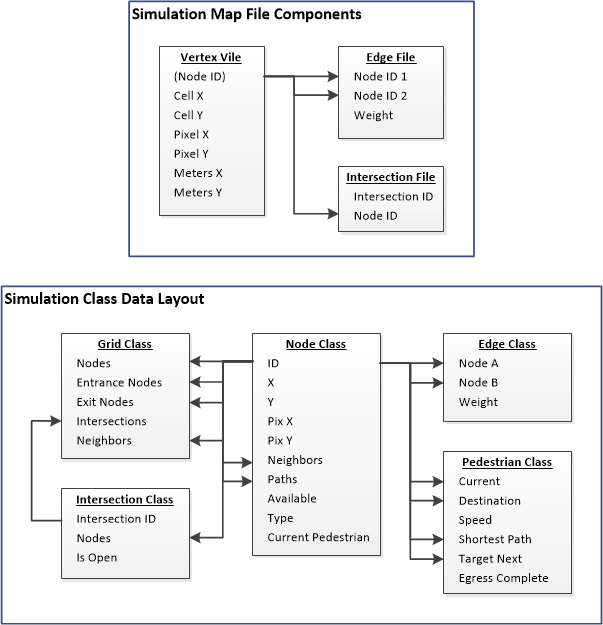
\includegraphics[width=\linewidth,natwidth=603,natheight=625]{DataLayout.png}
  \caption{Simulation Data Layout.}
  \label{fig:datalayout}
\end{figure}

\def\arraystretch{1.5}
\begin{table}
  \centering
    \begin{tabular}{p{0.5\linewidth}p{0.5\linewidth}}
     \hline
     Method & Description \\
     \hline
     Move(NewNode) & Takes one argument: a \textit{Node} object. When called,
                     marks the node set to \textit{Current} as unavailable,
                     sets the \textit{Current} attribute to NewNode,
                     and marks the NewNode object as unavailable. \\
     GetCurrentNode() \newline SetCurrentNode(CurrentNode) & Returns or sets
                        the current node that the pedestrian is occupying. \\
     GetDestinationNode() \newline SetDestinationNode(DestNode) & Returns or
                        sets the destination node for the pedestrian. \\
     GetTargetNext() \newline SetTargetNext(TargetNext) & Returns or
                       sets the target next node for the pedestrian in the
                       shortest path to his destination. \\
     GetEgressComplete() \newline SetEgressComplete(Complete) & Returns or
                        sets the current egress status of the pedestrian. True
                        once the pedestrian has exited the SUI, and false
                        otherwise. \\
     \hline
    \end{tabular}
    \caption{Methods of the \textit{Pedestrian} class.}
  \label{table:pedestrian_methods}
\end{table}

\subsubsection{Node Class Interfaces}
We define a \textit{Node} class as shown in Table \ref{table:node_methods}.
Nodes are the primary abstraction for the resource entities in the simulation,
which are sidewalks and roads. Nodes have several key attributes defined that
can be retrieved and set. Among them, the Neighbors attribute specifies all the
nodes that are one degree away from the node object. The Neighbors attribute is
then used to populate the \textit{Paths} attribute for the node, which is a hash map
that gives the shortest path to each possible destination node
in the simulation. We precompute the \textit{Paths} attribute for each entrance
node in the graph prior to beginning the simulation. This precomputation step
needs only be repeated when a parameter change occurs that alters the underlying
node structure or availability.

\def\arraystretch{1.5}
\begin{table}
  \centering
    \begin{tabular}{p{0.5\linewidth}p{0.5\linewidth}}
     \hline
     Method & Description \\
     \hline
     GetAvailable() \newline SetAvailable(Bool)  & Gets or sets the current
                        value of the \textit{Available} attribute for the node.
                        If the setter, must be a boolean true or false. \\
     GetPaths() \newline SetPaths(Paths) & Returns or sets the Paths attribute
                of the node, which is a hash map that gives the next node in
                the shortest path to each possible destination node in the
                simulation. \\
     GetNeighborNodes() \newline SetNeighborNodes(ListNodes) & Returns or sets
                        the Neighbors attribute of the node, corresponding to
                        the nodes one edge length away. If the setter, takes
                        one argument: list of \textit{Node} objects. \\
     GetNodeType() & Returns the NodeType Attribute of the node. \\
     GetNodeID() & Returns the NodeID Attribute of the node. \\
     \hline
    \end{tabular}
    \caption{Methods of the \textit{Node} class.}
  \label{table:node_methods}
\end{table}

\subsubsection{Intersection Class Interfaces}
Within our simulation, we utilize a number of intersections that are
parametrically closed and opened. Thus, we define key methods for the
\textit{Intersection} class in Table \ref{table:intersection_methods}.

Intersections are used to limit the rate of flow of pedestrians through the SUI,
increasing the reality of the simulation. As an intersection contains one or
more nodes, when an intersection is closed, all the nodes within it are
closed to additional pedestrian traffic. This means no new pedestrian traffic is
allowed into the intersection.  Pedestrians currently in the intersection as it
closes will not be able to move if their next node is within the intersection.
Although keeping pedestrians trapped in the middle of the road is unrealistic,
it simplifies the model and the effect on the simulation was decided to be
negligible as the same ``delay'' effect is still executed.

\def\arraystretch{1.5}
\begin{table}
  \centering
    \begin{tabular}{p{0.5\linewidth}p{0.5\linewidth}}
     \hline
     Method & Description \\
     \hline
     OpenMe()  & When called, sets the \textit{Available} attribute to
                 true for every node in its \textit{Nodes} array. Sets the
                 \textit{Open} attribute for the intersection to true. \\
     CloseMe() & When called, sets the \textit{Available} attribute to
                 false for every node in its \textit{Nodes} array. Sets the
                 \textit{Open} attribute for the intersection to false. \\
     GetNodes() & Returns the list of \textit{Node} objects that are part of the
                  intersection. \\
     SetNodes(ListNodes) & Takes one argument: list of \textit{Node} objects.
                           Sets the \textit{Node} objects that make up the
                           intersection. \\
     \hline
    \end{tabular}
    \caption{Methods of the \textit{Intersection} class.}
    \label{table:intersection_methods}
\end{table}

\section{Results}
As mentioned earlier, several intersections were identified in the SUI.  These
intersections are shown in Fig. \ref{fig:intersectionMap}.

Ten distinct combinations of intersection states were created with the purpose
of evaluating the time it takes for pedestrians to evacuate the SUI under each
combination; this is shown in Table \ref{table:configs}.  Green cells indicate
an intersection open exclusively for pedestrians and closed to vehicular traffic (i.e., it is effectively a sidewalk),
yellow cells indicate an intersection with alternating vehicular and pedestrian
traffic (i.e., a law enforcement officer directing traffic or a normal crosswalk), and red cells indicate
an intersection closed to all pedestrian traffic (i.e., nodes are removed from
the map).

\begin{table}[]
	\centering
	\resizebox{\columnwidth}{!}{%
		\begin{tabular}{clllllllllll}
			\multicolumn{1}{l}{}                                    &                                  & \multicolumn{10}{c}{Configuration \#}                                                                                                                                                                                                                                                                                                                                                                                                                                                                                                                     \\ \cline{3-12}
			\multicolumn{1}{l}{}                                    & \multicolumn{1}{l|}{}            & \multicolumn{1}{l|}{\textbf{1}}                     & \multicolumn{1}{l|}{\textbf{2}}                     & \multicolumn{1}{l|}{\textbf{3}}                     & \multicolumn{1}{l|}{\textbf{4}}                     & \multicolumn{1}{l|}{\textbf{5}}                     & \multicolumn{1}{l|}{\textbf{6}}                     & \multicolumn{1}{l|}{\textbf{7}}                     & \multicolumn{1}{l|}{\textbf{8}}                     & \multicolumn{1}{l|}{\textbf{9}}                     & \multicolumn{1}{l|}{\textbf{10}}                    \\ \cline{2-12}
			\multicolumn{1}{c|}{}                                   & \multicolumn{1}{l|}{\textbf{1}}  & \multicolumn{1}{l|}{\cellcolor[HTML]{32CB00}open}   & \multicolumn{1}{l|}{\cellcolor[HTML]{FFFC9E}normal} & \multicolumn{1}{l|}{\cellcolor[HTML]{32CB00}open}   & \multicolumn{1}{l|}{\cellcolor[HTML]{FFFC9E}normal} & \multicolumn{1}{l|}{\cellcolor[HTML]{32CB00}open}   & \multicolumn{1}{l|}{\cellcolor[HTML]{FFFC9E}normal} & \multicolumn{1}{l|}{\cellcolor[HTML]{32CB00}open}   & \multicolumn{1}{l|}{\cellcolor[HTML]{FFFC9E}normal} & \multicolumn{1}{l|}{\cellcolor[HTML]{FFFC9E}normal} & \multicolumn{1}{l|}{\cellcolor[HTML]{32CB00}open}   \\ \cline{2-12}
			\multicolumn{1}{c|}{}                                   & \multicolumn{1}{l|}{\textbf{2}}  & \multicolumn{1}{l|}{\cellcolor[HTML]{FFFC9E}normal} & \multicolumn{1}{l|}{\cellcolor[HTML]{32CB00}open}   & \multicolumn{1}{l|}{\cellcolor[HTML]{32CB00}open}   & \multicolumn{1}{l|}{\cellcolor[HTML]{FFFC9E}normal} & \multicolumn{1}{l|}{\cellcolor[HTML]{FFFC9E}normal} & \multicolumn{1}{l|}{\cellcolor[HTML]{32CB00}open}   & \multicolumn{1}{l|}{\cellcolor[HTML]{32CB00}open}   & \multicolumn{1}{l|}{\cellcolor[HTML]{FFFC9E}normal} & \multicolumn{1}{l|}{\cellcolor[HTML]{FFFC9E}normal} & \multicolumn{1}{l|}{\cellcolor[HTML]{FFFC9E}normal} \\ \cline{2-12}
			\multicolumn{1}{c|}{}                                   & \multicolumn{1}{l|}{\textbf{3}}  & \multicolumn{1}{l|}{\cellcolor[HTML]{FFFC9E}normal} & \multicolumn{1}{l|}{\cellcolor[HTML]{FD6864}closed} & \multicolumn{1}{l|}{\cellcolor[HTML]{FFFC9E}normal} & \multicolumn{1}{l|}{\cellcolor[HTML]{FFFC9E}normal} & \multicolumn{1}{l|}{\cellcolor[HTML]{FFFC9E}normal} & \multicolumn{1}{l|}{\cellcolor[HTML]{FD6864}closed} & \multicolumn{1}{l|}{\cellcolor[HTML]{32CB00}open}   & \multicolumn{1}{l|}{\cellcolor[HTML]{FFFC9E}normal} & \multicolumn{1}{l|}{\cellcolor[HTML]{FD6864}closed} & \multicolumn{1}{l|}{\cellcolor[HTML]{FD6864}closed} \\ \cline{2-12}
			\multicolumn{1}{c|}{}                                   & \multicolumn{1}{l|}{\textbf{4}}  & \multicolumn{1}{l|}{\cellcolor[HTML]{FFFC9E}normal} & \multicolumn{1}{l|}{\cellcolor[HTML]{FFFC9E}normal} & \multicolumn{1}{l|}{\cellcolor[HTML]{FFFC9E}normal} & \multicolumn{1}{l|}{\cellcolor[HTML]{FFFC9E}normal} & \multicolumn{1}{l|}{\cellcolor[HTML]{FFFC9E}normal} & \multicolumn{1}{l|}{\cellcolor[HTML]{FFFC9E}normal} & \multicolumn{1}{l|}{\cellcolor[HTML]{FFFC9E}normal} & \multicolumn{1}{l|}{\cellcolor[HTML]{FFFC9E}normal} & \multicolumn{1}{l|}{\cellcolor[HTML]{FFFC9E}normal} & \multicolumn{1}{l|}{\cellcolor[HTML]{FFFC9E}normal} \\ \cline{2-12}
			\multicolumn{1}{c|}{}                                   & \multicolumn{1}{l|}{\textbf{5}}  & \multicolumn{1}{l|}{\cellcolor[HTML]{32CB00}open}   & \multicolumn{1}{l|}{\cellcolor[HTML]{FFFC9E}normal} & \multicolumn{1}{l|}{\cellcolor[HTML]{FFFC9E}normal} & \multicolumn{1}{l|}{\cellcolor[HTML]{FFFC9E}normal} & \multicolumn{1}{l|}{\cellcolor[HTML]{32CB00}open}   & \multicolumn{1}{l|}{\cellcolor[HTML]{FFFC9E}normal} & \multicolumn{1}{l|}{\cellcolor[HTML]{32CB00}open}   & \multicolumn{1}{l|}{\cellcolor[HTML]{32CB00}open}   & \multicolumn{1}{l|}{\cellcolor[HTML]{FD6864}closed} & \multicolumn{1}{l|}{\cellcolor[HTML]{32CB00}open}   \\ \cline{2-12}
			\multicolumn{1}{c|}{}                                   & \multicolumn{1}{l|}{\textbf{6}}  & \multicolumn{1}{l|}{\cellcolor[HTML]{32CB00}open}   & \multicolumn{1}{l|}{\cellcolor[HTML]{FFFC9E}normal} & \multicolumn{1}{l|}{\cellcolor[HTML]{FD6864}closed} & \multicolumn{1}{l|}{\cellcolor[HTML]{FFFC9E}normal} & \multicolumn{1}{l|}{\cellcolor[HTML]{32CB00}open}   & \multicolumn{1}{l|}{\cellcolor[HTML]{FFFC9E}normal} & \multicolumn{1}{l|}{\cellcolor[HTML]{32CB00}open}   & \multicolumn{1}{l|}{\cellcolor[HTML]{32CB00}open}   & \multicolumn{1}{l|}{\cellcolor[HTML]{FFFC9E}normal} & \multicolumn{1}{l|}{\cellcolor[HTML]{32CB00}open}   \\ \cline{2-12}
			\multicolumn{1}{c|}{}                                   & \multicolumn{1}{l|}{\textbf{7}}  & \multicolumn{1}{l|}{\cellcolor[HTML]{FFFC9E}normal} & \multicolumn{1}{l|}{\cellcolor[HTML]{FFFC9E}normal} & \multicolumn{1}{l|}{\cellcolor[HTML]{FFFC9E}normal} & \multicolumn{1}{l|}{\cellcolor[HTML]{FFFC9E}normal} & \multicolumn{1}{l|}{\cellcolor[HTML]{FFFC9E}normal} & \multicolumn{1}{l|}{\cellcolor[HTML]{FFFC9E}normal} & \multicolumn{1}{l|}{\cellcolor[HTML]{FFFC9E}normal} & \multicolumn{1}{l|}{\cellcolor[HTML]{FFFC9E}normal} & \multicolumn{1}{l|}{\cellcolor[HTML]{FFFC9E}normal} & \multicolumn{1}{l|}{\cellcolor[HTML]{FFFC9E}normal} \\ \cline{2-12}
			\multicolumn{1}{c|}{}                                   & \multicolumn{1}{l|}{\textbf{8}}  & \multicolumn{1}{l|}{\cellcolor[HTML]{FFFC9E}normal} & \multicolumn{1}{l|}{\cellcolor[HTML]{FFFC9E}normal} & \multicolumn{1}{l|}{\cellcolor[HTML]{FFFC9E}normal} & \multicolumn{1}{l|}{\cellcolor[HTML]{FFFC9E}normal} & \multicolumn{1}{l|}{\cellcolor[HTML]{FFFC9E}normal} & \multicolumn{1}{l|}{\cellcolor[HTML]{FFFC9E}normal} & \multicolumn{1}{l|}{\cellcolor[HTML]{FFFC9E}normal} & \multicolumn{1}{l|}{\cellcolor[HTML]{FFFC9E}normal} & \multicolumn{1}{l|}{\cellcolor[HTML]{FFFC9E}normal} & \multicolumn{1}{l|}{\cellcolor[HTML]{FFFC9E}normal} \\ \cline{2-12}
			\multicolumn{1}{c|}{}                                   & \multicolumn{1}{l|}{\textbf{9}}  & \multicolumn{1}{l|}{\cellcolor[HTML]{FFFC9E}normal} & \multicolumn{1}{l|}{\cellcolor[HTML]{FD6864}closed} & \multicolumn{1}{l|}{\cellcolor[HTML]{FFFC9E}normal} & \multicolumn{1}{l|}{\cellcolor[HTML]{FFFC9E}normal} & \multicolumn{1}{l|}{\cellcolor[HTML]{FD6864}closed} & \multicolumn{1}{l|}{\cellcolor[HTML]{FFFC9E}normal} & \multicolumn{1}{l|}{\cellcolor[HTML]{FFFC9E}normal} & \multicolumn{1}{l|}{\cellcolor[HTML]{FFFC9E}normal} & \multicolumn{1}{l|}{\cellcolor[HTML]{FD6864}closed} & \multicolumn{1}{l|}{\cellcolor[HTML]{FFFC9E}normal} \\ \cline{2-12}
			\multicolumn{1}{c|}{}                                   & \multicolumn{1}{l|}{\textbf{10}} & \multicolumn{1}{l|}{\cellcolor[HTML]{FFFC9E}normal} & \multicolumn{1}{l|}{\cellcolor[HTML]{FFFC9E}normal} & \multicolumn{1}{l|}{\cellcolor[HTML]{FFFC9E}normal} & \multicolumn{1}{l|}{\cellcolor[HTML]{FFFC9E}normal} & \multicolumn{1}{l|}{\cellcolor[HTML]{FFFC9E}normal} & \multicolumn{1}{l|}{\cellcolor[HTML]{FFFC9E}normal} & \multicolumn{1}{l|}{\cellcolor[HTML]{FFFC9E}normal} & \multicolumn{1}{l|}{\cellcolor[HTML]{FFFC9E}normal} & \multicolumn{1}{l|}{\cellcolor[HTML]{FFFC9E}normal} & \multicolumn{1}{l|}{\cellcolor[HTML]{FFFC9E}normal} \\ \cline{2-12}
			\multicolumn{1}{c|}{}                                   & \multicolumn{1}{l|}{\textbf{11}} & \multicolumn{1}{l|}{\cellcolor[HTML]{FFFC9E}normal} & \multicolumn{1}{l|}{\cellcolor[HTML]{FFFC9E}normal} & \multicolumn{1}{l|}{\cellcolor[HTML]{FFFC9E}normal} & \multicolumn{1}{l|}{\cellcolor[HTML]{FFFC9E}normal} & \multicolumn{1}{l|}{\cellcolor[HTML]{FFFC9E}normal} & \multicolumn{1}{l|}{\cellcolor[HTML]{FFFC9E}normal} & \multicolumn{1}{l|}{\cellcolor[HTML]{FFFC9E}normal} & \multicolumn{1}{l|}{\cellcolor[HTML]{FFFC9E}normal} & \multicolumn{1}{l|}{\cellcolor[HTML]{FFFC9E}normal} & \multicolumn{1}{l|}{\cellcolor[HTML]{FFFC9E}normal} \\ \cline{2-12}
			\multicolumn{1}{c|}{\multirow{-12}{*}{\rotatebox{90}{Intersection ID}}} & \multicolumn{1}{l|}{\textbf{12}} & \multicolumn{1}{l|}{\cellcolor[HTML]{FFFC9E}normal} & \multicolumn{1}{l|}{\cellcolor[HTML]{FFFC9E}normal} & \multicolumn{1}{l|}{\cellcolor[HTML]{FFFC9E}normal} & \multicolumn{1}{l|}{\cellcolor[HTML]{FFFC9E}normal} & \multicolumn{1}{l|}{\cellcolor[HTML]{FFFC9E}normal} & \multicolumn{1}{l|}{\cellcolor[HTML]{FFFC9E}normal} & \multicolumn{1}{l|}{\cellcolor[HTML]{FFFC9E}normal} & \multicolumn{1}{l|}{\cellcolor[HTML]{FFFC9E}normal} & \multicolumn{1}{l|}{\cellcolor[HTML]{FFFC9E}normal} & \multicolumn{1}{l|}{\cellcolor[HTML]{FFFC9E}normal} \\ \cline{2-12}
		\end{tabular}%
	}
	\caption{Intersection Configurations}
	\label{table:configs}
\end{table}

Intersection configurations were carefully configured to adhere to two governing
rules:

\begin{enumerate}
  \item Intersections on North Ave shall never be open (i.e., closed to vehicular
traffic).
  \item No closed intersections shall make any destination node unreachable.
\end{enumerate}

To achieve statistical significance, 20 runs were performed per intersection
configuration.  As stated earlier, 90\% confidence intervals were constructed
from each set of 20 runs.  The plot of the expected value, along with error
bars representing the 90\% confidence intervals, is shown in Fig.
\ref{fig:evacuationtimes}.  The runs are sorted such that the lowest expected
evacuation times increase from left to right.

\begin{figure}[H]
  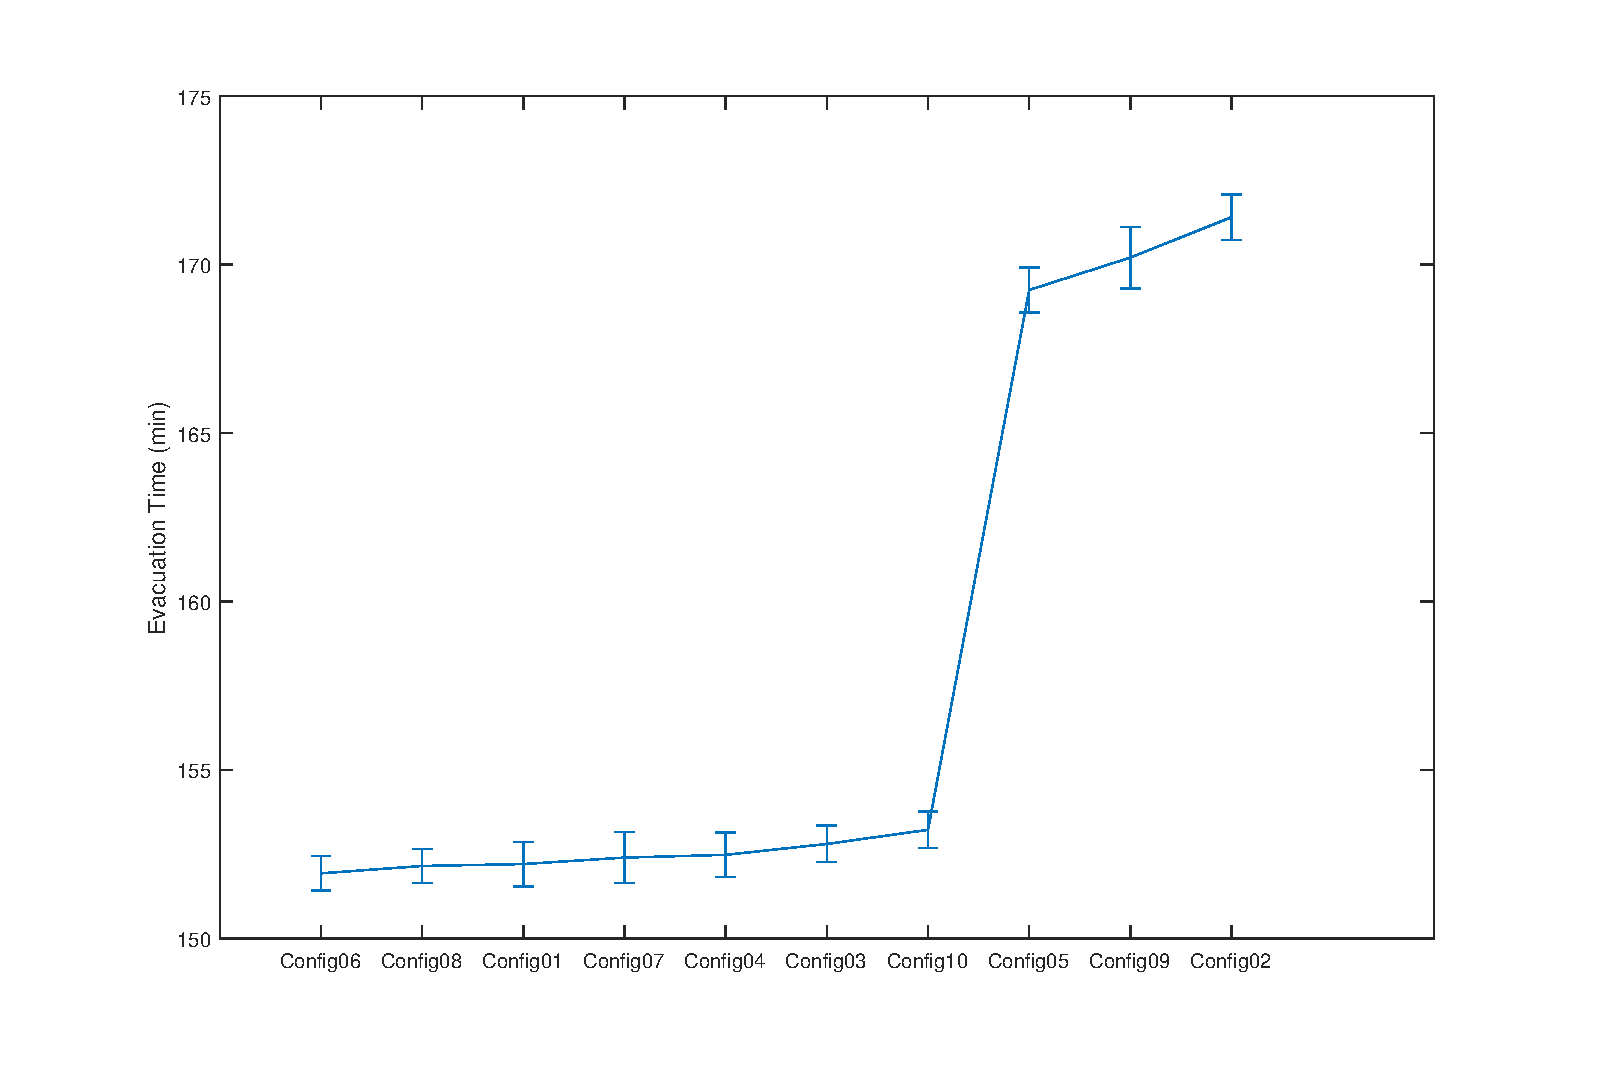
\includegraphics[width=\linewidth,natwidth=1002,natheight=662]{EvacuationTimes.eps}
  \caption{SUI Evacuation Times.}
  \label{fig:evacuationtimes}
\end{figure}

There are a few takeaways from the parametric results above.  First, the
step-like behavior in evacuation times is caused exclusively by the closure of
intersection 9; this is one of the few pathways that cross North Avenue.
According to the results, its closure leads to an increase in average evacuation
time by roughly 15 minutes.  The second takeaway is that, aside from the state
of intersection 9 (which is never green, as this would violate the rule of
not closing North Avenue to vehicular traffic), the state of other intersections
do not have a statistically significant impact to evacuation time.  Finally,
the 90\% confidence intervals are not very large: the maximum interval was merely
0.9118 minutes, indicating the expected values plotted are, at worst, 90\% likely
to be within about 1 minute of the true mean of each configuration's random variable.

An example of the impact of closing intersection 9 follows. Consider configuration 2
and configuration 6; note that the only difference between these two configurations
is the state of intersection 9. Similarly, configuration 5 and configuration 1
exhibit this same relationship.  In Fig. \ref{fig:evacuationtimes}, note that
configurations 2 and 5 turned out to be on the upper portion of the step-like
function, while configurations 6 and 1 are on the lower portion; this lends
further validity to the notion that the closure of intersection 9 is indeed
the only culprit (in the set of tested intersection configurations) of longer
evacuation times observed in the simulation runs.

\subsection{Verification Methodoogy}
Throughout development of the model, team members routinely reviewed code
that they did not write; this ensured that outside perspectives and fresh
sets of eyes reviewed the code.  Code is very modular and compartmented to avoid
a multitude of programmatic pitfalls.

Before running on the SUI depicted in Fig. \ref{fig:polygon}, a smaller map
was generated to evaluate model execution on a much smaller scale (the smaller
map featured 2,380 nodes, while the SUI investigated in this study contained
107,498 nodes). This facilitated rapid identification and fixing of bugs in
a scalable simulation, and instilled confidence that the simulation was running
as expected on the larger map.

Visualization was a critical aspect of verifying the simulation model, and
the development team regularly reviewed recordings of visualizations, in
addition to carrying out real-time visual inspection of runs as they happened.

Addressing the soundness of the vertex, edge, and intersection files, sanity
checks were performed to avoid common pitfalls (such as edges referencing
nodes that do not exist and intersections referencing nodes not representing
roadways). One-wayness of map file generation also precluded tool-related
bugs if one wanted to change these entities.

As described earlier, goodness-of-fit tests were employed to ensure random
number generation was satisfactorally performed.

\subsection{Validation Methodology}
Literature of comparable pedestrian simulations with similar outputs (i.e.,
evacuation time analyses) was extensively used to define details regarding
our model. A comprehensive description of takeaways from literature may be
found in Section \ref{sec:literature}.

As specified earlier, the pedestrian interarrival time was derived
experimentally by observing a crowd of pedestrians exiting a structure. The
data from this was scaled to meet the size of the exits in our particular SUI.

The evacuation times themselves were evaluated based upon each author's
experiences, which provides a level of face validation. In addition,
configurations expected to have higher evacuation times (such as configuration
9, which had the most closed intersections) and lower evacuation times
(configuration 7, with the most open intersections) were identified, and the
results aligned with this intuition.

Again, visualization was utilizaed to ensure the simulation of pedestrian
motion matched the authors' expectations based on real-world experiences.

Finally, only practical intersection configurations were evaluated, where a practical
intersection is defined as adhering to the governing rules listed earlier.

\section{Conclusion}
While the closure of intersection 9 (shown in Fig. \ref{fig:intersectionMap})
to pedestrians appears to be responsible for an approximate 15 minute increase
in evacuation time (raising the evacuation time from 2.5 hours to 2.75 hours),
this amounts to an approximate 10\% increase in evacuation time from the SUI
as compared to when intersection 9 is operating like a conventional crosswalk.

For the intersection configurations tested, there was not a single configuration
that stood out as a configuration that yields significantly lower evacuation
times relative to the other configurations.  As such, so long as pedestrians are able
to arrive at their destinations, under the assumptions noted in this paper,
there is no evidence of a superior configuration which dramatically reduces
evacuation time.

\section{Final Notes}
It should be noted that all of the authors contributed equally to this work.
From a testing perspective, our simulation model has been tested primarily in
a Mac OS X environment - specifically, OS X 10.11.3 with Python 2.7.

Thanks are due to the TAs and instructor for their assistance with our many
questions.

\clearpage
\bibliography{template}{}
\bibliographystyle{plain}
\end{document}
